\section{Results}
\label{results}
We divide our evaluation into six parts. Firstly, we run the automatically labeling algorithm iteratively and show the change of the performance. Secondly, we will examine the importance of different features in the SVM classifier. Thirdly, we compare the accuracy of our final classifier with other several baseline classifiers (HMM, CRF and pattern-based), the difference caused by the difference training set will also be shown. Fourthly, we evaluate the effect of enlarging the drug and ADR lexica. Finally, we evaluate the accuracy of discovered ADRs with the help of drug package inserts, and show the top-ten discovered ADRs of several drugs, as verification and supplement for the known ADRs in the package inserts.

\subsection{Impact of the iteration}
\label{subsec:3.1}
\begin{figure}
\centering
	\includegraphics[width=0.6\columnwidth]{Fig3.eps}
	\caption{F1-score, accuracy and training data size of the new SVM classifier at 
each iteration}
	\label{fig:3}       % Give a unique label
\end{figure}

Fig.~\ref{fig:3} shows the accuracies and F1-scores on the tuning set after each iteration, using the bootstrapping approach in Section~\ref{subsec:2.3}. The result at iteration 0 is obtained using only the manually labeled data. After each iteration, the training set will enlarge, however the speed of growth becomes slow in each iteration and drops to 0 at 15$^{th}$ iteration. By using the tuning set which contains 400 manually labeled data (200 positive + 200 negative) to calculate the f1-score and accuracy of our SVM classifier in each iteration, we observe quick convergence: the two values keep constant after 9$^{th}$ iteration. 

The biggest improvement of performance comes from the 0$^{th}$ iteration to the 
1$^{st}$ iteration since the most knowledge is acquired in the first round of 
bootstrapping. The gain in accuracy and f1-score saturates after a peak is reached at 
the 5$^{th}$ iteration. We therefore use the training data obtained at that time to 
train our final SVM classifier and other baseline classifiers.

\subsection{The effectiveness of classification features}
\label{subsec:3.2}

\begin{table}
	\centering
	\caption{The effectiveness of classification features}
	\label{tab:3}       % Give a unique label
	% For LaTeX tables use
%	\begin{tabular}{lllllll}
	\begin{tabular}{m{2.5cm}m{1.4cm}m{1.4cm}m{0.8cm}m{0.8cm}m{0.8cm}m{1cm}}
		\hline\noalign{\smallskip}
		SVM Features & positive pairs & negative pairs & R & P & F1 & accuracy \\
		\noalign{\smallskip}\hline\noalign{\smallskip}
		All & 184/200 & 148/200 & 0.92 & 0.78 & \textbf{0.844} & \textbf{0.830} \\
		without feature 1 & 175/200 & 152/200 & 0.875 & 0.785 & 0.827* & 0.818 \\
		without feature 2 & 184/200 & 147/200 & 0.92 & 0.776 & 0.842 & 0.828 \\
		without feature 3 & 175/200 & \textbf{153}/200 & 0.875 & \textbf{0.789} & 0.829* & 0.820 \\
		without feature 4 & \textbf{187}/200 & 144/200 & \textbf{0.935} & 0.770 & \textbf{0.844} & 0.828 \\
		without feature 5 & 169/200 & 131/200 & 0.845 & 0.710 & 0.772* & 0.750 \\
		without feature 6 & 180/200 & 141/200 & 0.900 & 0.753 & 0.820* & 0.803 \\
		without feature 7 & 173/200 & 146/200 & 0.865 & 0.762 & 0.810* & 0.798 \\
		\noalign{\smallskip}\hline
	\end{tabular}
\end{table}

To examine the contribution of each feature of our SVM classifier, we use the previous tuning set which contains 400 manually labeled sentences to performed ablation tests on the tuning set. The result is shown in Table~\ref{tab:3}. Compared with All features set, those significant changes (the difference of F1-score is more than 0.10) are marked with asterisks. Besides, the highest values in each column are highlighted in bold.

We find that each feature does the contribution for the performance of the classifier. Among all the features, feature 1, 3, 5, 6, 7 are the most important ones as F1-score decreases sigificantly without these features.

\subsection{Drug-ADR association}
\label{subsec:3.3}

\begin{table}
	\centering
	\caption{Performance of various classifier}
	\label{tab:4}       % Give a unique label
	% For LaTeX tables use
	%	\begin{tabular}{lllllll}
	\begin{tabular}{m{3cm}m{1.2cm}m{1.2cm}m{1.2cm}m{1.2cm}m{1.2cm}}
		\hline\noalign{\smallskip}
		Methods & positive pairs & negative pairs & Recall & Precision & F1-score \\
		\noalign{\smallskip}\hline\noalign{\smallskip}
		Manual labels (Pattern-based) & 24/100 & 97/100 & 0.24 & \textbf{0.889} & 0.378 \\
		Manual labels (HMM) & 62/100 & 85/100 & 0.62 & 0.805 & 0.700 \\
		Manual labels (CRF) & 86/100 & 75/100 & 0.86 & 0.775 & 0.815 \\
		Manual labels (SVM) & 68/100 & 87/100 & 0.68 & 0.840 & 0.751 \\
		Auto labels from inserts (Pattern-based) & 47/100 & 77/100 & 0.47 & 0.671 & 0.553 \\
		Auto labels from inserts (HMM) & 85/100 & 55/100 & 0.85 & 0.654 & 0.739 \\
		Auto labels from inserts (CRF) & 98/100 & 32/100 & \textbf{0.98} & 0.590 & 0.737 \\ 
		Auto labels from inserts (SVM) & 81/100 & 65/100 & 0.81 & 0.698 & 0.75 \\
		Semi-supervised labels (Pattern-based) & 76/100 & 89/100 & 0.76 & 0.874 & 0.813 \\
		Semi-supervised labels (HMM) & 87/100 & 54/100 & 0.87 & 0.654 & 0.747 \\
		Semi-supervised labels (CRF) & 98/100 & 34/100 & \textbf{0.98} & 0.598 & 0.742 \\
		Semi-supervised labels (SVM) & 86/100 & 79/100 & 0.86 & 0.804 & \textbf{0.831} \\	 
		\noalign{\smallskip}\hline
	\end{tabular}
\end{table}

According to the previous research, we use the training data obtained at the 5$^{th}$ iteration and all the features to train our SVM classifier. To make the comparison with several baseline classifiers, another 200 manually-labeled test data (100 positive + 100 negative), which are different from the previous tuning set, is chosen to check the performance of the various classifier. The result is shown in Table~\ref{tab:4}. There are three kinds of training data:

\begin{itemize}
	\item \textbf{Manual labels:} use the manually labeled training set with 300 positive instances and 300 negative instances
	\item \textbf{Auto labels from insert:} use the  training data that we obtained according to the package insert directly without help of the manually labeled data. If the symptom in the sentence is ADR according to the package insert, it will be added into positive training set. Inversely, if the symptom in the sentence is indication according to the package insert, it will be added into negative training set. 
	\item \textbf{Semi-supervised labels:} use the training data that we obtained after the 5$^{th}$ iteration.
\end{itemize}

The pattern-based classifier depends a lot on the size of the training data set. More training data could help it to recognize more patterns of a positive sentence. In consequence, the performance improves a lot when using semi-supervised labels.

The HMM-based classifier emphasizes on the structure of sentences. The performance improved if the structure in training set and testing set is standard. Therefore, when we use the manually-labeled data to train the HMM classifier, the small size of training data set results in a low precision. It can be also seen that the percentage of true positives is inversely correlated with the percentage of true negatives. This means a classifier is biased to produce either more positive labels or more negative labels. A good classifier, such as the one trained with the semi-supervised labels manages to strike a balance between the two biases and produce a better overall F1-score.

CRF-based classifier use the sequence labeling with word embedding cluster features, which reduces the effect of the training set’s size. However, this kind of classifier also depends on the grammatical form of a sentence. When training set enlarges, the structure of negative instances becomes various and do not have a regular form, which leads to a bad performance of the CRF classifier.

In short, both the HMM and CRF concentrate more on the information of the single word itself and its limited surrounding words. However, SVM focus on the features of the whole sentence.

The semi-supervised data, which is doubly verified by the primary SVM classifier and package inserts, may not have a very standard form (e.g., some sentences do not have the causal keyword but have a lot of noisy words between the ADR and its associated drug). For those user posts, which do not have a standard form, SVM performs clearly better because of its global view, and HMM doesn’t perform as well because it requires sentences in their standard form.

\subsection{Homophone transformation and extended ADR lexicon}
\label{subsec:3.4}

\begin{table}
	\centering
	\caption{Enlarging data set through homophone transform}
	\label{tab:5}       % Give a unique label
	% For LaTeX tables use
	%	\begin{tabular}{lllllll}
	\begin{tabular}{m{2cm}m{1.2cm}m{1.2cm}m{1.2cm}m{1.2cm}m{1.2cm}}
		\hline\noalign{\smallskip}
		& 倍他乐克 (Betaloc) & 耐信 (Nexium) & 拜唐苹 (Glucobay) & 氨茶碱 (Aminophylline) & All 79 drugs \\
		\noalign{\smallskip}\hline\noalign{\smallskip}
		official name & 24073 & 6521 & 530 & 7493 & 158695 \\
		homophone & 13177 & 6369 & 1611 & 2388 & 143485 \\
		total & 37250 & 12890 & 2141 & 9881 & 302180 \\
		\%increase & 35.4\% & 49.4\% & 75.2\% & 24.2\% & 47.5\% \\ 
		\noalign{\smallskip}\hline
	\end{tabular}
\end{table}

As shown in Table~\ref{tab:5}, our data set, measured by the number of sentences containing at least one of the 4 selected drugs and an ADR, is enlarged significantly after homophone transformation.

Among all the 302,180 sentences which contains a (drug, ADR) pair, there are totally 1,328 sentences where the candidate ADR contains an adverb of degree and can only be extracted by using the extended ADR lexicon. Although 1,328 is not large compared to 302,180, extended ADR lexicon could also help us to enlarge the data set to find more potential ADRs.

In addition, we randomly select 100 original posts to assess the 
quality of our ADR lexicon. Among all the 451 medications mentioned, 
we could detect 159 medications. After calculation, we obtain the precision 
and recall of our ADR lexicon is 1.0 and 0.353. Although there are still 
a number of undetected colloquial medications, we have tried our best 
to combine lexicons from sources(see Section~\ref{subsubsec:2.1.2}) and add 
the colloquial term(see Section~\ref{subsubsec:2.1.3}).  

\subsection{End-to-end ranking}
By using the ranking method which is referred in Section~\ref{subsec:2.5}, our system returns a ranked list of possible ADRs when given a drug. We evaluate the end-to-end performance of the system by the Average Precision ($AveP$) according to the package insert of the drug:

\begin{equation}
\label{equ:1}
	AveP = \frac{\sum_{k=1}^n (P(k)\times rel(k))}{number\;of\;ADRs\;in\;package\;inserts}
\end{equation}

where $P(k)$ is the precision at cut-off $k$ in the list, $rel(k)$ is an indicator function equaling 1 if the item at rank $k$ is a relevant document, 0 otherwise.\footnote{$AveP$ is defined at https://en.wikipedia.org/wiki/Information\_retrieval}

We expect the true ADR of a drug to rank high in the list while the true indication ranks lower in the list. The ground truth we use here is the known ADRs and known indications of four random-sampled drugs according to the package inserts. Figure 4 shows the results of the four previous randomly chosen drugs, 倍他乐克(\textit{Betaloc}), 耐信(\textit{Nexium}), 拜唐苹(\textit{Glucobay}) and 氨茶碱(\textit{Aminophylline}). We also calculate the weighted average of $AveP$ for all the 79 drugs.

\begin{figure}
	\centering
	% Use the relevant command to insert your figure file.
	% For example, with the graphicx package use
	\includegraphics[width=0.6\columnwidth]{Fig4.eps}
	%	\resizebox{0.8\hsize}{!}{\includegraphics*{firstFig1-01.eps}}
	%	\includegraphics{firstFig1-01.eps}
	% figure caption is below the figure
	\caption{End-to-end rankings’ AveP}
	\label{fig:4}       % Give a unique label
\end{figure}

From Fig.~\ref{fig:4}, we can see that $AveP(ADR)$ is much larger than $AveP(Indication)$, which means that most of ADRs that our classifier discovers are already included in the package insert. Besides, the known indications are not in our returned ADR list or ranked very low in our list.

Together with Table~\ref{tab:5}, which gives the sizes of the datasets for four drugs, we learn that more data helps to increase the ADR prediction accuracy.

\subsection{Top-ten discovered ADRs}
\label{subsec:3.6}

\newcommand{\tabincell}[2]{\begin{tabular}{@{}#1@{}}#2\end{tabular}}
\begin{table}
	\centering
	\caption{Top 10 discovered ADRs for 4 common drugs}
	\begin{tabular}{p{1cm}p{2cm}p{2cm}p{2cm}p{2cm}}
		\toprule
		\multicolumn{1}{l}{\tabincell{c}{\textbf{药物}\\ \textbf{(Drugs)}}} & \tabincell{c}{\textbf{倍他乐克} \\ \textbf{(Betaloc)}} & \tabincell{c}{\textbf{耐信}\\\textbf{(Nexium)}} & \tabincell{c}{\textbf{拜唐苹} \\ \textbf{(Glucobay)}} & \tabincell{c}{\textbf{氨茶碱 }\\\textbf{(Aminophylline)}} \\
		\midrule
		\multicolumn{1}{l}{\multirow{10}[2]{*}{\tabincell{c}{\textbf{副作用}\\\textbf{(ADRs)}}}} & \uline{咳嗽(2.45\%) (Cough)} & 咳嗽(1.77\%) (Cough) & \uline{不适(3.31\%) (Discomfort)} & \uline{咳嗽(51.39\%) (Cough)} \\
		& \uline{紧张(2.06\%) (Nervous)} & 头晕(1.09\%) (Dizziness) & \uline{无力(2.18\%) (Acratia)} & \uline{头晕(0.69\%) (Dizziness)} \\
		& \uline{不适(4.04\%) (Discomfort)} & 不适(2.30\%) (Discomfort) & \uline{发热(1.48\%) (Fever)} & 恶心(0.57\%) (Nausea) \\
		& 心悸(2.82\%) (Palpitation) & 紧张(0.32\%) (Nervous) & \uline{头晕(2.70\%) (Dizziness)} & \uline{心悸(0.26\%) (Palpitation)} \\
		& 头晕(5.52\%) (Dizziness) & 便秘(0.85\%) (Constipation) & \uline{乏力(1.31\%) (Weak)} & 呕吐(1.13\%) (Emesis) \\
		& 疲劳(0.67\%) (Fatigue) & \uline{疲劳(0.16\%) (Fatigue)} & \uline{瘙痒(0.87\%) (Itching)} & 心动过速(0.19\%) (Tachycardia) \\
		& 头痛(1.32\%) (Headache) & 失眠(0.50\%) (Insomnia) & 腹泻(1.13\%) (Diarrhea) & 心律失常(0.26\%) (Arrhythmia) \\
		& 恶心(0.89\%) (Nausea) & 头痛(0.36\%) (Headache) & \uline{低血糖(3.14\%) (Hypoglycemia)} & \uline{打鼾(0.22\%) (Snore)} \\
		& 便秘(0.16\%) (Constipation) & \uline{心悸(0.11\%) (Palpitation)} & \uline{虚弱(0.52\%) (Asthenia)} & 抽搐(0.22\%) (Tic) \\
		& \uline{瘙痒(0.14\%) (Itching)} & \uline{皮肤过敏(0.12\%) (Skin allergy)} & \uline{咳嗽(0.61\%) (Cough)} & \uline{紧张(0.12\%) (Nervous)} \\
		\bottomrule
	\end{tabular}%
	\label{tab:6}%
\end{table}%


Table~\ref{tab:6} shows the top-ten discovered ADRs for 4 aforementioned drugs. The percentage in the parentheses is calculated as followed:
\begin{equation}
	percentage = \frac{\#\;of\;patients\;who\;report\;that\;ADR}{\#\;of\;posts\;which\;discuss\;this\;drug}
\end{equation}

ADRs which don’t have direct match in the package inserts (therefore potentially new discoveries) are marked using {\em underline}.

In Table~\ref{tab:6}, we discovered many ADRs that are already included in the package inserts. Although these ADRs are known, the frequency statistics can be valuable for: i) verifying ADRs listed in the package inserts; ii) studying the relative frequency between the ADRs. For example, the frequency of \textit{Fatigue} and \textit{Constipation} of \textit{Betaloc} in package insert are both larger than 1\%, but they are 0.67\% and 0.16\% respectively in our result.

There are also a number of ADRs without direct match in the manuals. These fall into several cases:
\paragraph{Newly discovered ADRs} (e.g., “咳嗽(Cough)” for “倍他乐克(\textit{Betaloc})”). This is the most valuable discovery for the drug maker in the analysis of the drug reactions because some ADRs may not be observed during the trials 
on a small population. 
\paragraph{Synonyms of the known ADRs} (e.g., “疲乏(Exhaustion)” is a synonym of “疲劳(Fatigue)” for “耐信(\textit{Nexium}) ”.  While they are synonyms, the ADRs listed in package inserts are often some terminologies and the colloquial synonyms can help patients understand them easily.
\paragraph{Generalization of the known ADRs} (e.g., “呕吐(Emesis)” is a specialization of the symptom “不适 (Discomfort)” for “倍他乐克 (\textit{Betaloc})”). Some ADRs from package inserts is a specific symptom. Our results give a general term.

